\section{Cel shading}
Som beskrevet i afsnit 1 'Introduktion' opnås Cel shading ved f.eks. at optegne karaktere med sorte streger, et eksempel kan ses på figur \ref{fig:jetsetradio2000}, hvor den samme karakter er repræsentateret to gange. Henholdsvis med og uden brug af cel shading. Selv om karakterne er fra samme spil og derfor er lige gamle, virker karakteren til højre væsentlige nyere og meget pænere end karakteren til venstre. 

\pic{h}{15em}{Files/CelShading/jetsetradio.pdf}{Sammenligning af figur fra Jet Set Radio, hvor man tydeligt kan se de sorte streger på karakteren til højre}{fig:jetsetradio2000}Cel shading kan ikke kun opnås ved, at tegne på computeren. Man kan nemlig gøre det gennem programmering, i f.eks. OpenGL. Koden vil ikke blive vist og vil ikke blive forklaret, men den bagved liggende proces vil. Hjemmesiden Sunandblackcat \cite{sunandblackcat2016} har en beskrivelse af cel shading, samt en gennemgang af kode, som kan bruges til shading, beskivelse af processen laves med udgangspunkt af denne gennemgang.\\
Før der kan laves en silouet skal man rendere en mesh. Det gør man ved, at bruge en shader som tilføjer en konstant farve for hver renderet fragment og skifter hver spids af mesh’en langs normalen, med en konstant værdi som er størrelsen af silhuetten.\\ Her bør man tillade rendering af ’Back-Faces’.\footnote[1]{Front/back faces bruges til at beskrive polygoner}

Dernæst visualisere man den samme mesh igen, men normalen sættes til 0 og den konstante farve skiftes til hvid.  Dernæst skal man deaktivere skrivning til dybde buffer og aktivere visualisering af ’Front-Faces’. Dernæst kan man gå videre til farve reduktion. Det er værd at bemærke at det andet ’Draw call’ ikke er nødvendigt, hvis man også benytter sig at farve reduktion. 
Man kan beregne hver komponent af lyse (ambient, diffuse and specular) and tilføje dem sammen. Dernæst kan man finde total værdien af clamp.\footnote[2]{Engelsk begreb for en matematisk operation}

Med denne værdi er det muligt, at få en 1D texture som indeholder et sæt af farver for cel shading. Antallet af farver på cel shading er det samme som antallet af farver på teksturen. Det skal bemærkes, at cel shading effekten kan opnås uden brug af intensitet på farve teksturen. 
Man kan definere base farven, for cel shading og få delmængden af den totale intensitet.Formlen for, at opnå dette ses i (\ref{shadeIntensity})
\matharray{shadeIntensity = ceil(intensity * numShades)/numShades}{shadeIntensity}
 
\matharray{finalColor = baseColor * shadeIntensity} {modulationbasecolor} 
%\pic{ht}{15em}{Files/CelShading/silhouette4}{Modulation med grund farver}{fig:modulationbasecolor}
%\wrapfigure{L}{15em}{Files/CelShading/silhouette4.pdf}{Modulation med grund farver}{fig:modulationbasecolor}
%\begin{wrapfigure}{l}{0.3\textwidth}
%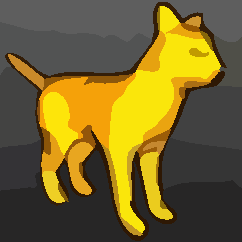
\includegraphics{Files/CelShading/silhouette4.pdf} 
%\caption{This is a figure caption.}
%\end{wrapfigure}
\wrapfig{l} {10em}{Files/CelShading/silhouette4.pdf} {Modulation med grund farver} {fig:modulationbasecolor}


Intensiteten kan bruges til, at ændre base farven for cel shadingen. Formlen for dette ses i \ref{modulationbasecolor} og resultatet ses i figur \ref{fig:modulationbasecolor}. 
Hvis den brugte mesh, er ubestemt/ansigtsløs kan man ændre farven ud fra teksturen/intensiteten. 
\matharray{finalcolor = modelTexture * shadeIntensity} {modulationofcolorfromteksture}
Formel og resultat kan ses ved henholdsvis (\ref{modulationofcolorfromteksture})og figur \ref{fig:modulationofcolorfromteksture}. Sidst, men ikke mindst kan man bruge en blanding fra de to forrige eksempler, hvor man både bruge base farve, teksture og intensitet. Formelen ses i \ref{mixedmodulation} og resultatet ses i figur \ref{fig:mixedmodulation}.
\matharray{finalcolor = baseColor * modelTexture * shadeIntensity} {mixedmodulation}
\newpage\pic{h}{15em}{Files/CelShading/silhouette5.pdf}{Ændring af farve på baggrund af tekstur}{fig:modulationofcolorfromteksture}

\pic{h}{15em}{Files/CelShading/silhouette6.jpg}{Modulation med grund farver og tekstur } {fig:mixedmodulation}
 
